\documentclass[default,iicol]{sn-jnl}

\usepackage{amsmath}
\usepackage{array}
\usepackage[acronym]{glossaries}
\usepackage{epsfig} %% for loading postscript figures
\usepackage{float}
\usepackage[utf8]{inputenc}
\usepackage{siunitx}
\usepackage{stfloats}
\usepackage{subfig}
\usepackage{titlesec}
\usepackage{url}
\usepackage{xcolor}

% get rid of colon for tables and figures as requested per journal format
\usepackage[labelsep=space]{caption}

\setcounter{secnumdepth}{4}

\titleformat{\paragraph}
{\normalfont\normalsize\bfseries}{\theparagraph}{1em}{}
\titlespacing*{\paragraph}
{0pt}{3.25ex plus 1ex minus .2ex}{1.5ex plus .2ex}

%\def\url#1{\expandafter\string\csname #1\endcsname}
\newcounter{exno}
\newenvironment{examples}
{
\begin{flushleft}
\begin{tabular}{>{(\refstepcounter{exno}\theexno\label{row:\theexno}) }rl}
}
{
\end{tabular}
\end{flushleft}
}
%\newcommand*{\@rowstyle}{}
\newcommand*{\rowstyle}[1]{% sets the style of the next row
  \gdef\@rowstyle{#1}%
  \@rowstyle\ignorespaces%
}
\newcolumntype{=}{% resets the row style
  >{\gdef\@rowstyle{}}%
}
\newcolumntype{+}{% adds the current row style to the next column
  >{\@rowstyle}%
}
\definecolor{ao}{rgb}{0.0, 0.5, 0.0}
\definecolor{coolblack}{rgb}{0.0, 0.18, 0.39}

\glsdisablehyper
\newacronym[longplural={centers of mass}]{com}{CoM}{center of mass}
\newacronym[longplural={equations of motion}]{eom}{EoM}{equation of motion}
\newacronym{ocp}{OCP}{optimal control problem}
\newacronym{grf}{GRF}{ground reaction force}
\newacronym{vgrf}{VGRF}{vertical ground reaction force}
\newacronym{nlp}{NLP}{non-linear programming problem}
\newacronym[longplural={degrees of freedom}]{dof}{DoF}{degree of freedom}
\newacronym{rfd}{RFD}{rate of force development}
\newacronym{cmj}{CMJ}{countermovement jump}

% \usepackage{fancyhdr}% http://ctan.org/pkg/fancyhdr

% % \fancyhf{}% Clear header/footer
% % \fancyhead[R]{\sectionmark}
% % \fancyfoot[C]{\thepage}% \fancyfoot[R]{\thepage}
% % \renewcommand{\headrulewidth}{0.4pt}% Default \headrulewidth is 0.4pt

% % \renewcommand{\sectionmark}[1]{\markright{\thesection~- ~#1}}
% % \renewcommand{\chaptermark}[1]{\markboth{\chaptername~\thechapter~-~ #1}{}}
% \renewcommand{\subsectionmark}[1]{\markright{#1}}

% %\usepackage[T1]{fontenc}
% \usepackage{bold-extra}


% % % Fancyhdr setup
% % \pagestyle{fancy}% Change page style to fancy
% % \fancyhf{} % clear all header fields
% % \fancyhead[L]{\footnotesize\scshape\leftmark}
% % \fancyhead[R]{\footnotesize\scshape\rightmark}
% % \fancyfoot[C]{\thepage}
% % \renewcommand{\headrulewidth}{0.4 pt}
% % \renewcommand{\footrulewidth}{0 pt}

\newcounter{magicrownumbers}
\newcommand\rownumber{\stepcounter{magicrownumbers}\arabic{magicrownumbers}}
\newcommand\figwidth{174mm}

\jyear{2021}%

\raggedbottom
%%\unnumbered% uncomment this for unnumbered level heads

\begin{document}

\title[Optimal Skateboard Geometry for Maximizing Ollie Height]{
  Optimal Skateboard Geometry for Maximizing Ollie Height}

%%=============================================================%%
%% Prefix	-> \pfx{Dr}
%% GivenName	-> \fnm{Joergen W.}
%% Particle	-> \spfx{van der} -> surname prefix
%% FamilyName	-> \sur{Ploeg}
%% Suffix	-> \sfx{IV}
%% NatureName	-> \tanm{Poet Laureate} -> Title after name
%% Degrees	-> \dgr{MSc, PhD}
%% \author*[1,2]{\pfx{Dr} \fnm{Joergen W.} \spfx{van der} \sur{Ploeg} \sfx{IV} \tanm{Poet Laureate} 
%%                 \dgr{MSc, PhD}}\email{iauthor@gmail.com}
%%=============================================================%%

\author*[1]{\fnm{Jan T.} \sur{Heinen}}\email{janheinen97@gmail.com}

\author[1]{\fnm{Samuel G.} \sur{Brockie}}\email{s.g.brockie@tudelft.nl}

\author[1]{\fnm{Raymund} \sur{ten Broek}}\email{raymund@uspc.nl}

\author[1]{\fnm{Eline} \sur{van der Kruk}}\email{e.vanderkruk@tudelft.nl}

\author[1]{\fnm{Jason K.} \sur{Moore}}\email{j.k.moore@tudelft.nl}

\affil*[1]{\orgdiv{Department of Biomechanical Engineering}, \orgname{TU Delft}, \orgaddress{\street{Leeghwaterstraat}, \postcode{2628 CN}, \city{Delft}, \country{Netherlands}}}

\abstract{The most basic skateboarding trick is called
the ollie. The athlete jumps up while pushing down on the back end of the
skateboard’s tail, causing a rotation about the back axle. The upward
acceleration due to the rotation together with the tail-ground impact cause
the skateboard to go airborne while dragging the skateboard up with the feet.  To reach maximum height the dynamics such as impact, dynamic response, and torque production are dependent on shape, inertia and mass, which gives reason to assume an optimal shape exists. This leads to the research question: What are the
optimal geometric and inertial parameters of a skateboard for an Olympic
athlete to reach maximal ollie height. The skateboard geometry is optimized
through multiphase direct collocation with the objective of maximal ollie
height. Modelling the dynamics of the ollie including impact and friction are done with a point mass human controller that is kineticly and kinematicly mapped to a counter movement jump. A simplistic contact implicit impact scheme is made for a higher order optimization. The ollie height is improved by changing the mass and inertia properties of the skateboard.  Multiple optimal board shapes are generated for example a skateboard with a smaller wheelbase can reach higher ollie
height compared to an industry standard skateboard.
}

\keywords{Skateboarding, Optimal Control, Parameter Optimization, Direct Collocation}
\maketitle

\section{Introduction}\label{s_intro}

In 1978 Alan `Ollie' Gelfand invented the `no-hand aerial', by riding off an inclined surface and jumping in the air with a skateboard.
Four years later, Rodney Mullen debuted the first ollie from flat ground.
Because the skateboard is not tethered to the skater, an ollie requires a precise sequence of movements to keep the two together~\cite{frederick_biomechanics_2006}.
The maneuver can be deconstructed into the six
distinct phases shown in Fig.~\ref{fig:ollie steps}.

\begin{figure*}[!t]
\captionsetup[subfigure]{labelformat=empty}
  \subfloat[$t_1$=0.013]{{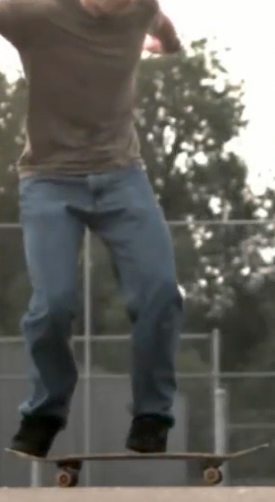
\includegraphics[width=0.13\textwidth]{figure/1.png} }}%
  \subfloat[$t_2$=0.129]{{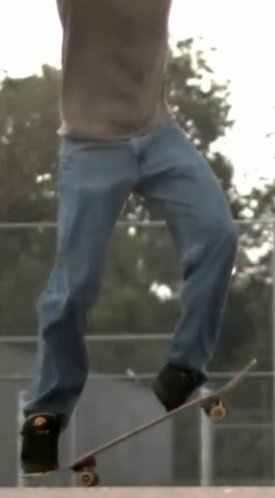
\includegraphics[width=0.13\textwidth]{figure/2.png} }}%
  \subfloat[$t_3$=0.181]{{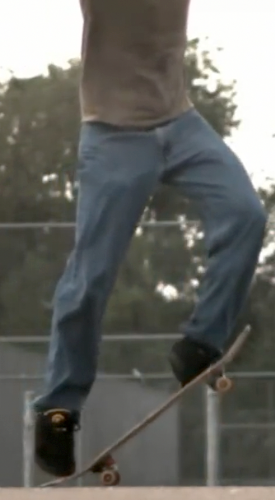
\includegraphics[width=0.13\textwidth]{figure/3.png} }}%
  \subfloat[$t_4$=0.187]{{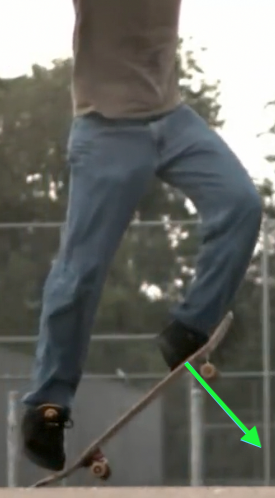
\includegraphics[width=0.13\textwidth]{figure/4.png} }}%
  \subfloat[$t_5$=0.303]{{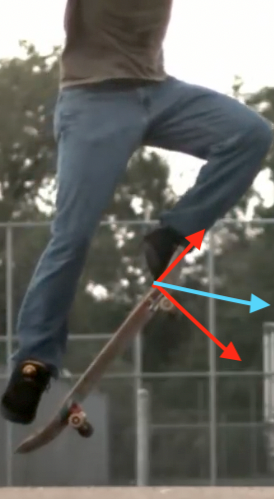
\includegraphics[width=0.13\textwidth]{figure/5.png} }}%
  \subfloat[$t_6$=0.431]{{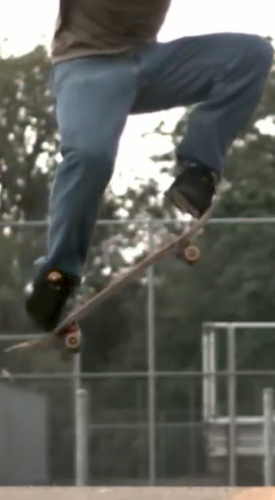
\includegraphics[width=0.13\textwidth]{figure/6.png} }}%
  \subfloat[$t_7$=0.543]{{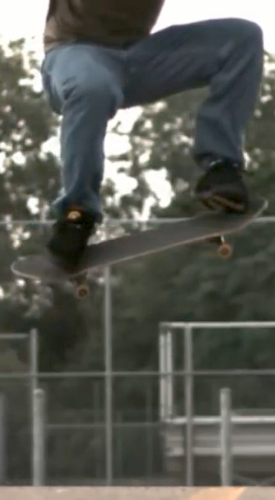
\includegraphics[width=0.13\textwidth]{figure/7.png} }}%
  \protect\newline
  \centering
  \subfloat[$t_8$=0.676$^1$]{{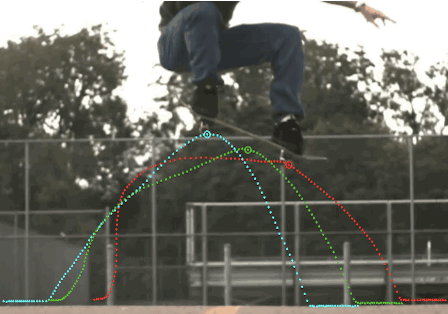
\includegraphics[width=0.336\textwidth]{figure/ollie_tracking_mid.png} }}
  \subfloat[$t_9$=0.722]{{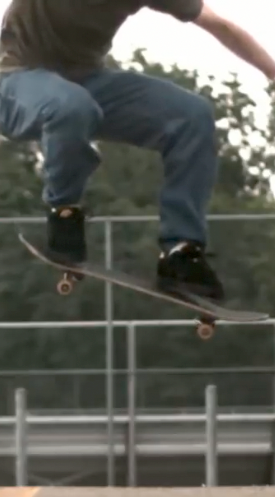
\includegraphics[width=0.13\textwidth]{figure/9.png} }}%
  \subfloat[$t_{10}$=0.904]{{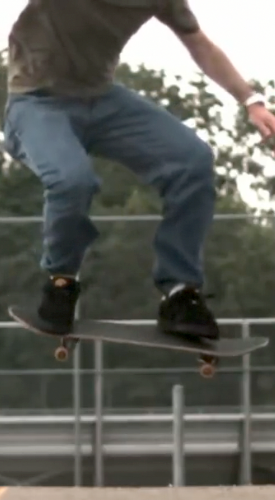
\includegraphics[width=0.13\textwidth]{figure/10.png} }}%
  \subfloat[$t_{11}$=1.097]{{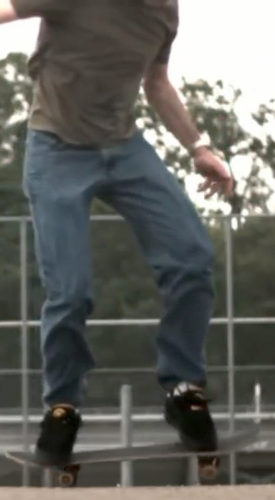
\includegraphics[width=0.13\textwidth]{figure/11.png} }}%
  \captionsetup{singlelinecheck=off}
\footnotesize
    \begin{center}
    \begin{tabular}{p{1.4cm} p{0.75cm} p{12.5cm}}
        \toprule
        Phase & Motion Cue & Description \\
        \midrule
        Preparation     & $t_1$ & The skater lowers their \gls{com} preparing to jump \\
        Pre-pop         & $t_2$ & The skater pushes firmly from their back leg and is decreasing downward force on the front foot, which results in the front wheels leaving the ground, simultaneously sliding the front foot forward \\
        Pop             & $t_3$ & Tail collides with the ground, the front foot is still sliding and the back foot is barely in contact with the skateboard~\cite{determan_kinetics_2006,nakashima_simulation_2021} \\
        Upward motion   & $t_4$ & Back foot is no longer in contact with the skateboard, the back wheels are not in contact with the ground anymore~\cite{determan_kinetics_2006,nakashima_simulation_2021} \\
                        & $t_5$ & The front foot reached the nose of the skateboard \\
                        & $t_6$ & Back foot contacts the board again \\
                        & $t_7$ & Board is leveled out by the front foot \\
                        & $t_8$ & Highest point is reached. Knees are fully tucked in, the biomechanical obstruction restricts the board from gaining height. Feet are firmly placed on the deck \\
        Downward motion & $t_9$ & Front foot loses contact \\
                        & $t_{10}$& Board is horizontal, both feet are in contact \\
        Landing         & $t_{11}$& The back wheels touch the ground and legs are almost fully stretched out \\
        \bottomrule
    \end{tabular}
    \end{center}
 \caption[Ollie motion cues]{
    Green arrow: resultant force without friction, red arrows: force components
    with friction, blue arrow: resultant force with friction. Blue-, green- and
    red line are trajectory of back wheel, middle and front wheel respectively. Images are retrieved from \url{youtu.be/339k4XEvbxY} with consent
  }
  \label{fig:ollie steps}
\end{figure*}

From the early 1960s, new skateboarding pursuits and their differing performance requirements evolved a variety of skateboard shapes.
For example, slalom demanded short boards for quick turns, downhill preferred longboards for stability, and pool skating resulted in wide, concave boards for maximum foothold. 
Artistic motives shaped impractical coffin- and
fish-like boards~\cite{prentiss_get_2011}.
The prevailing modern board shape, used by all Olympic athletes, is the popsicle stick.
The shape supports freestyling, where the ollie is a foundational trick.

There is no standardization of boards in the skateboard industry.
Boards are measured differently by each brand~\cite{johnny_skateboarding_2013} and non-specific descriptions such as mellow, steep, and wide are usually used to communicate deck dimensions to customers~\cite{berger_handmade_2021}.
This makes it difficult for skaters to find their optimal board shape.

Skaters know and feel when a specific skateboard performs to their liking.
However, they do not know how this translates to quantifiable dimensions.
Skateboards might have evolved to optimum geometries over the years, but from an academic and mechanical point of view, skateboard designs have not been shown to be optimal for specific tricks.

Researchers analyze the skateboard in planar riding models~\cite{hubbard_lateral_1979,hubbard_human_1980,kremnev_nonlinear_2010,ispolov_skateboard_1996,rosatello_skateboard_2015,varszegi_stability_2017,varszegi_stabilizing_2016,varszegi_downhill_2016,varszegi_balancing_2014,kuleshov_mathematical_2007,kuleshov_various_2010}, which show the relationship between the dimensions and the stability while rolling and turning. 
However, these dimensional analyses do not apply to aerial movements like the ollie.
Others research the ollie by investigating the contact forces~\cite{anderson_ollie_2020,shield_contact-implicit_2022} and biomechanics~\cite{frederick_biomechanics_2006,vorlicek_analysis_2015,wood_3d_2020,nakashima_simulation_2021,nevitt_ground_2006,candotti_lower_2012,dias_using_2016,anderson_ollie_2020,bridgman_human_1992,ou_postural_2021}.
Two papers have optimized the ollie without changing the geometry~\cite{anderson_ollie_2020,shield_contact-implicit_2022}, but no research has yet shown how the skateboards' dimensions influence the ollie.
Such research would benefit the skateboarding community.

Now that skateboarding is an Olympic sport, knowing how to improve performance is more important then ever.
Achieved height is the most measurable Olympic judging criteria applicable to the ollie~\cite{world_skate_skateboarding_2021}.
This leads to the research question:
\begin{quote}
\textit{
    What are the optimal geometric parameters of a skateboard for an Olympic athlete to reach maximal ollie height?}
\end{quote}

\subsection{Skateboard Terminology}
A labeled diagram of a popsicle stick skateboard is shown in Fig.~\ref{fig:skateboard terminology}. 
Additionally, the skateboard front will always be presented on the right-hand side and the riding direction will be assumed as left to right.

\begin{figure}[t]
    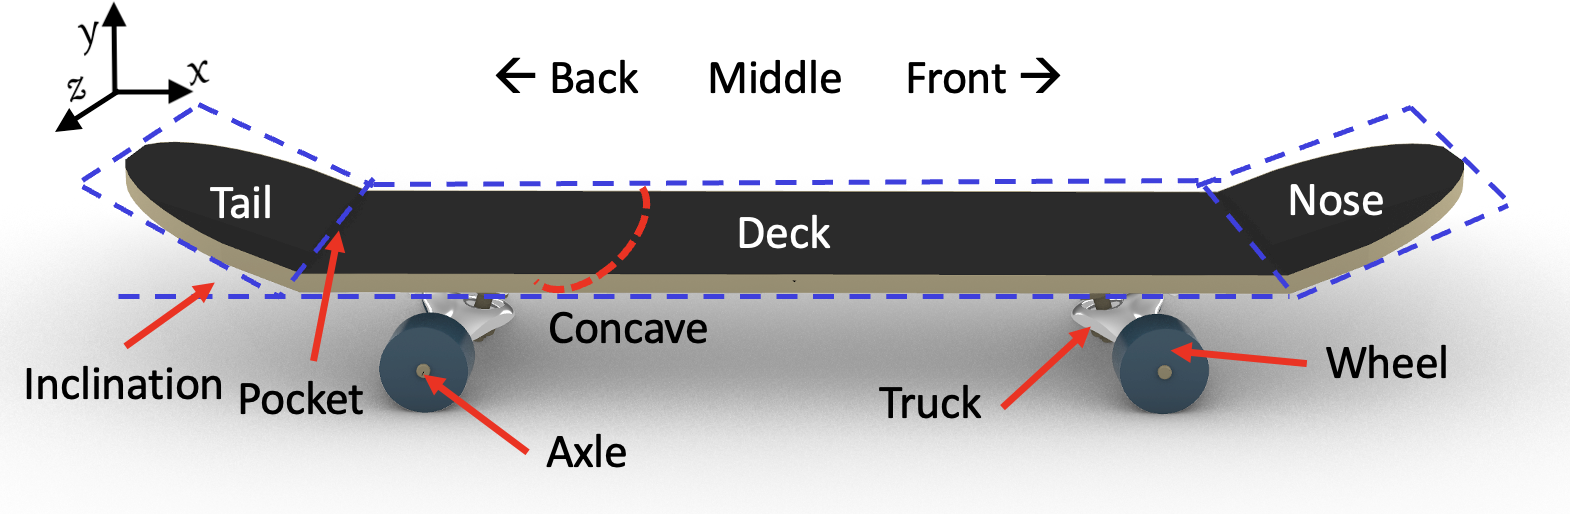
\includegraphics[width=0.5\textwidth]{figure/terminology.png}
    \caption[Skateboard terminology]{Skateboard terminology}
    \label{fig:skateboard terminology}
\end{figure}

\subsection{Mechanics of the ollie} \label{ss_mechanics}
Fig.~\ref{fig:ollie steps} details 11 motion cues ($t_1-t_{11}$) observed during an ollie, found by analysing a slow-motion video.

Friction occurs between the feet and the griptape due to the force normal to the board exerted by the feet together with sliding movement tangential to the surface.
This benefits ollie height because the resultant force (Fig.~\ref{fig:ollie steps} $t_5$, blue arrow) is directed more vertically upwards than the normal force (Fig.~\ref{fig:ollie steps} $t_4$, green arrow), which results in less downward motion while leveling out the skateboard mid air.
The higher the coefficient of friction between the foot and the deck, the more upward the resultant force will be.
That is why griptape on the deck and rubber-soled shoes is the choice of preference among skaters.

Impact is also important in the mechanics of an ollie.
An impulsive impact between the tail and the ground causes the `pop', which changes the translational and angular velocities of the board, causing it lose contact with the ground and move upwards.

\section{Method}

\subsection{Geometry and Parameterization}\label{s_paropt}
The most widely used modern skateboard is the popsicle stick skateboard. We simplify the popsicle stick skateboard design for our 2D model with an assumption about nose-tail symmetry and by ignoring the deck concavity, and describe it with ten variables. The variables colored blue in figure~\ref{fig:parameterized skateboard} while the variables colored green are set to an industrial standard. $d_{tr}$, $d_d$ and $d_w$, do not change the geometry of the skateboard model in the 2D plane of interest. $h_d$ does influence the skateboard mass and inertia properties. However, the same effect of changing deck height can also be achieved by keeping $h_d$ constant and varying $r_w$ or $h_{tr}$, which is desirable as this model does not take into account board stiffness.

%%%%%%%%%%%%%%%% begin figure %%%%%%%%%%%%%%%%%%%
\begin{figure}
  \centerline{
    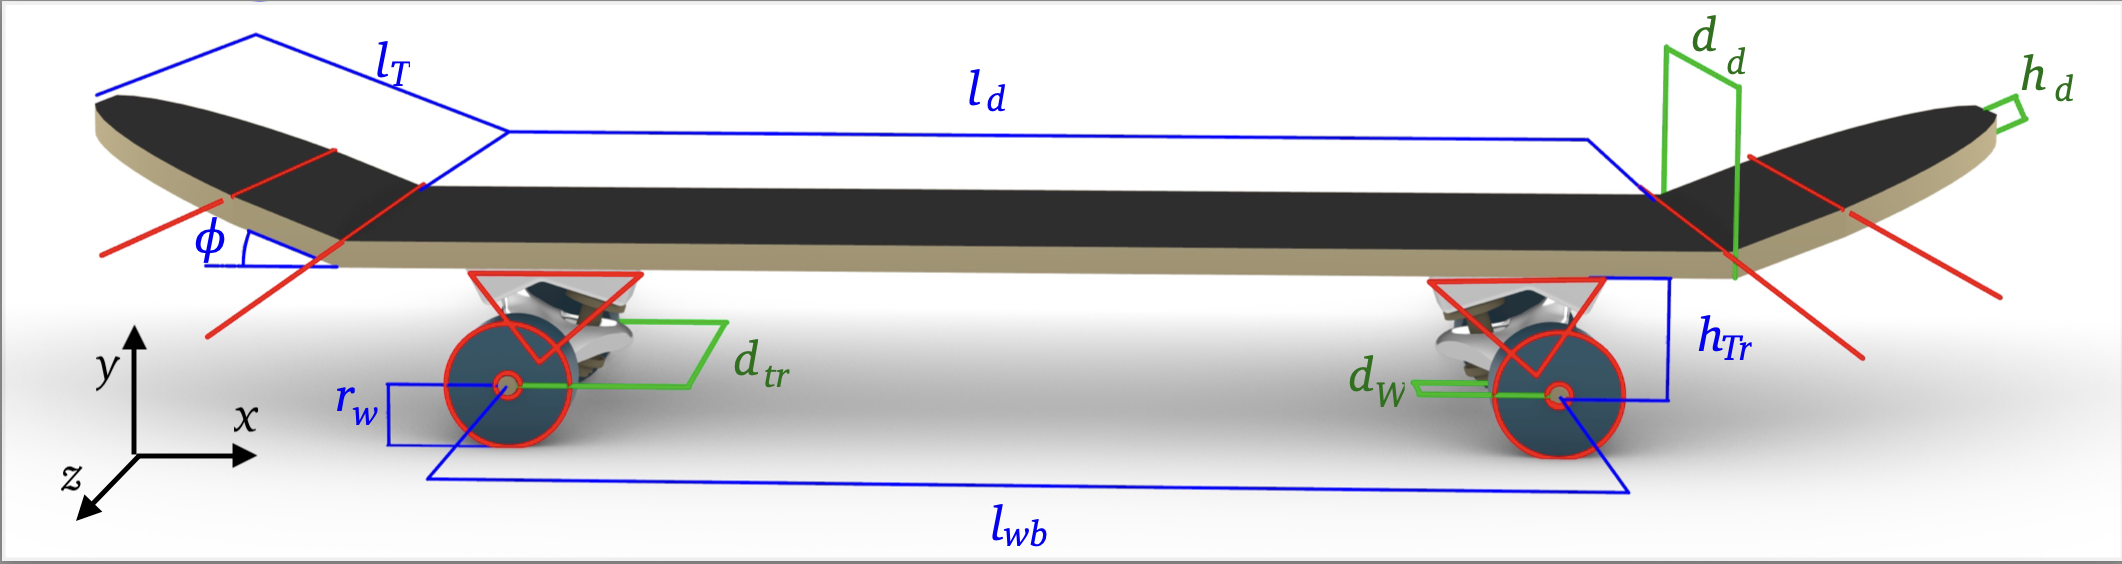
\includegraphics[width=0.5\textwidth,trim={0.1cm 0.1cm 0.1cm 0.05cm},clip]{figure/parameterized.png}
  }
  \footnotesize
  \begin{center}
  \begin{tabular}{=l +l +c}
    \toprule
    \rowstyle{\textbf}& Variable & Description \\
    \midrule
    \rowstyle{\color{blue}} & $l_{wb}$ & Wheelbase \\
    \rowstyle{\color{blue}} & $l_{d}$ & Deck length \\
    \rowstyle{\color{blue}} & $l_{t}$ & Tail/nose length \\
    \rowstyle{\color{blue}} & $\phi$ & Tail/nose inclination \\
    \rowstyle{\color{blue}} & $h_{tr}$ & Truck height \\
    \rowstyle{\color{blue}} & $r_{w}$ & Wheel radius \\
    \rowstyle{\color{ao}} & $h_d$ & Deck thickness \\
    \rowstyle{\color{ao}} & $d_{tr}$ & Truck width \\
    \rowstyle{\color{ao}} & $d_{d}$ & Deck width \\
    \rowstyle{\color{ao}} & $d_w$ & Wheel width \\
    \rowstyle{\color{orange}} & $d_{com}$ & COM distance from deck \\
    \bottomrule
  \end{tabular}
  \end{center}
  \caption{Parameterized skateboard. Blue parameters are optimized, green parameters are set to industrial standard. Orange is a dependent on other variables. Red lines split the skateboard into 11 basic shaped segments for inertia calculation}
\label{fig:parameterized skateboard}
\end{figure}
%%%%%%%%%%%%%%%% end figure %%%%%%%%%%%%%%%%%%%

We developed a mass and inertial model, which is a function of the skateboard's essential geometry, and material densities (wood, steel, urethane). The model is made up of eleven basic constant density shapes shown in Fig.~\ref{fig:parameterized skateboard}.

\subsection{Optimal Control Problem}
We formulate an \gls{ocp} with the objective of maximising the peak board height during the ollie. This is a simultaneous trajectory optimization of the board's dynamics and control, and parameter optimization of its geometric parameters. We use a direct method as they are well-suited for when dynamics and control must be computed to a similar accuracy and the structure of the control trajectory is not known a priori~\cite{kelly_introduction_2017}. We make use of Pycollo~\cite{brockie_predictive_2021} to numerically solve the \gls{ocp}. Pycollo solves the generalized multi-phase \gls{ocp} described in \citet{betts_practical_2010} by transcribing the \gls{ocp} to a \gls{nlp} using an LGL (Legendre-Gauss-Lobatto) collocation method~\cite{betts_using_2016}. The \gls{nlp} is then solved using Ipopt~\cite{biegler_large-scale_2009}. Pycollo also ph-mesh refinement~\cite{patterson_ph_2015} to iteratively improve the transcription mesh, solving successive \glspl{nlp} until a desired solution tolerance is met.

\subsection{Phases and Objective} \label{s_phases}

We use a multi-phase formulation for the ollie \gls{ocp} to handle discontinuities in the state trajectories in a numerically-stable manner. This allows, for example, the impact of the tail with the ground during the pop to be treated as an impulse, which is not possible during a single continuous phase. A disadvantage of this approach however is that the transition between phases is prescribed, leaving no room for the optimizer to discover these transitions. The three dynamically-distinct phases are:
\begin{enumerate} \label{n_phases}
  \item Preparation phase
  \item Upward motion
  \item Downward motion
\end{enumerate}

During the preparation phase the back wheels are in contact with the ground. The tail impact with the ground defines the transition from preparation to the upward motion. During upward and downward motion nothing is in contact with the ground and they both are governed by the same \glspl{eom}. We split the upward motion and downward motion into two phases because Pycollo requires that the objective function be a function of initial or final state variables of a phase~\cite{brockie_predictive_2021}. The transition from upward to downward motion defines the highest ollie.

To  define the maximum height achieved during the ollie, we constrain the board to be level at the highest point and
take the height achieved to be the middle of a fictional tangent touching lowest point of both wheels. The objective function for maximization is:
%
\begin{equation}
  \mathcal{J} = y_s^{(2)}(t_F) + d_{com} - h_{tr} - r_w
\end{equation}

\noindent where $y_s^{(2)}(t_F)$ is the height achieved by the skateboard's \gls{com} at the end of the second phase, $d_{com}$ is the distance between the skateboard's \gls{com} and the deck.

\subsection{System Dynamics}\label{s_systemdynamics}

\subsubsection{Skateboard Equations of Motion}
While in reality a skateboard bends and flexes during the ollie, this study assumes a rigid body model of the skateboard to reduce mathematical complexity.

The skateboard model is detailed in Fig.~\ref{fig:FBD}. In phase 1 we use a sliding joint for the rear wheel contact to eliminate the ground reaction forces from the \glspl{eom}.
During phase 2 and 3 the skateboard is an unconstrained rigid body in 2D. 

\begin{figure}
    \centering
    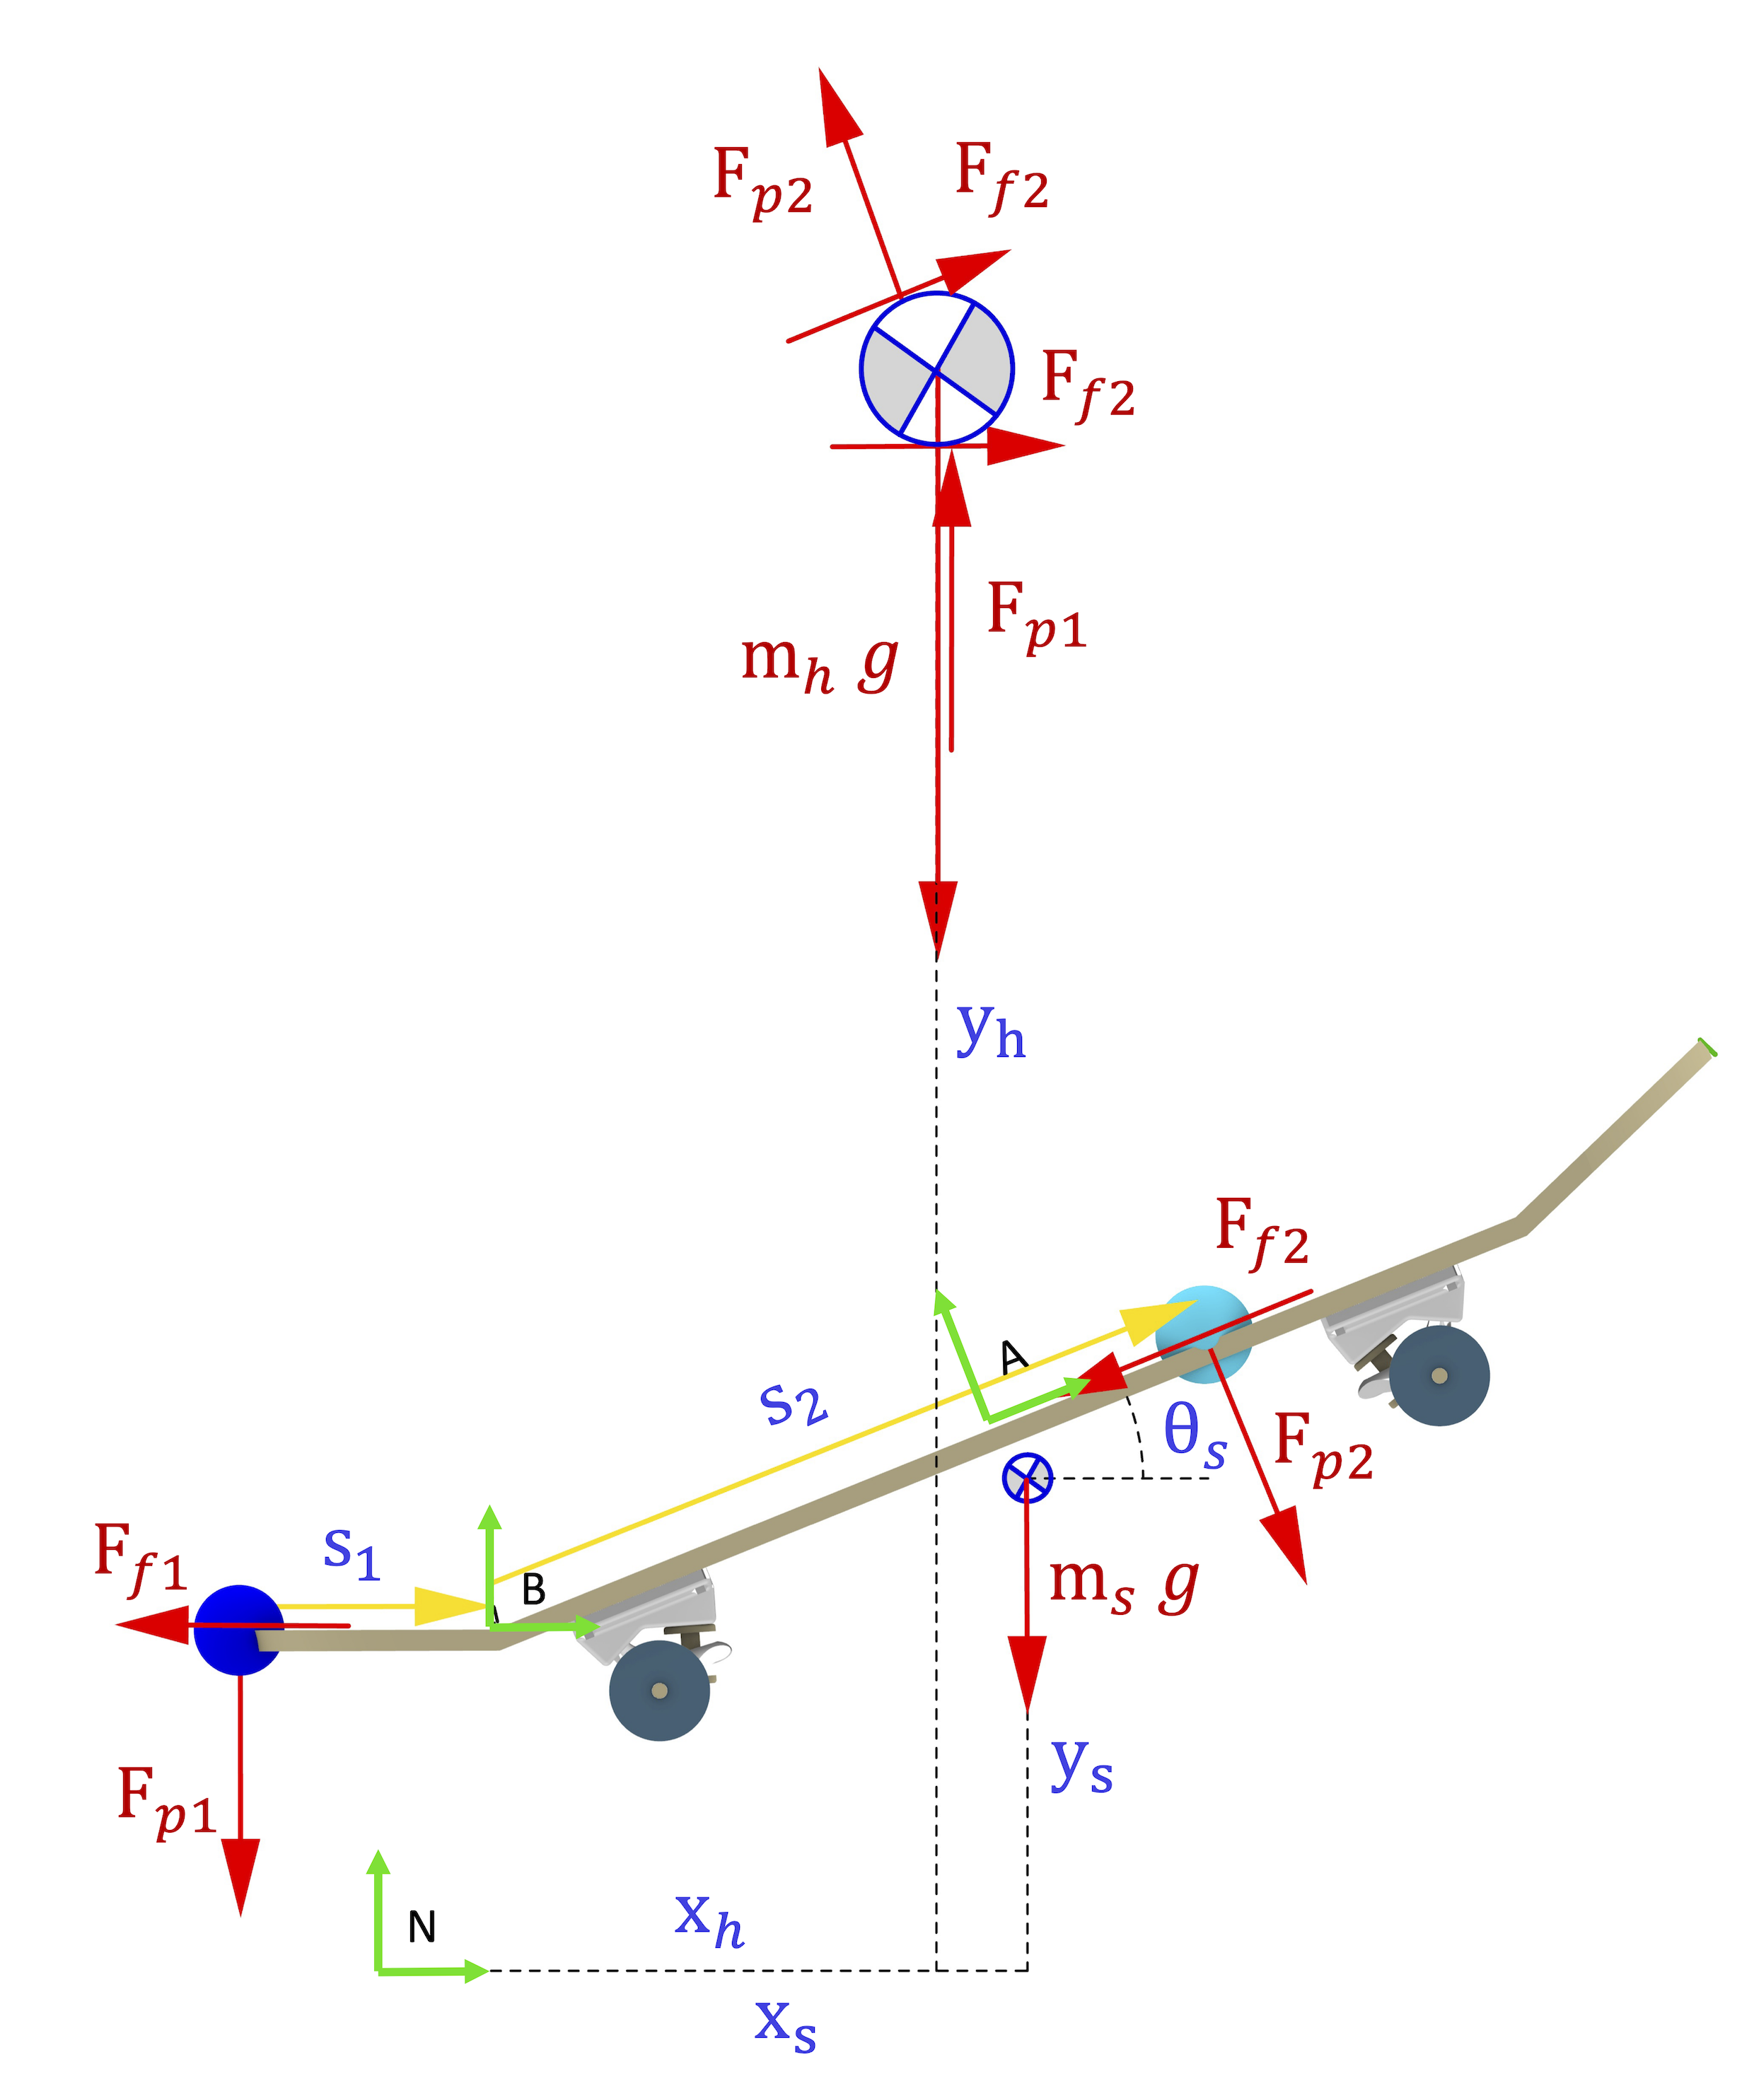
\includegraphics[width=0.45\textwidth]{figure/FBD_skater_feet.png}
    \footnotesize\begin{tabular}{|l l|l l|} \hline
    \color{blue}Blue: & State variables &\color{red} Red: & Forces \\ \hline
    \color{cyan}Cyan dot: & Front foot & \color{blue}Blue dot: & Back foot \\ \hline
    \color{yellow}Yellow: & Foot movement & \color{green}Green: & Frames \\ \hline
    \end{tabular}
    \caption[Free Body Diagrams phase 2 and 3]{Free body diagrams of human and skateboard for phase 1. $N$ is the inertial frame, and $A$ and $B$ are body fixed frames. Forces acting between the feet and human's \gls{com} are equal and opposite}
    \label{fig:FBD}
\end{figure}

\subsubsection{Human Equations of Motion}
The human is represented by a point mass on top of the skateboard, again detailed in Fig.~\ref{fig:FBD}.
The interactions between the point mass and the skateboard are modeled as a pair of equal and opposite forces acting between the massless feet and the human's \gls{com}.
Due to this simplification, this model does not represent metabolic leg power, only the mechanical power output~\cite{van_der_kruk_power_2018,morin_biomechanics_2018}. Inertia of the human's body segments is neglected.

We derive the \glspl{eom} using the TMT method~\cite{vallery_heike_advanced_2018}, facilitated by SymPy~\cite{meurer_sympy_2017}.
The code used for the derivation is provided in \cite{heinen_optimal_2022}, along with a mathematical description of the \glspl{eom}.

\subsection{Constraints}

\subsubsection{Human Model}

We constrain the kinetics and kinematics of the human to compensate for the simplifications used.

Musculoskeletal restrictions bound the kinematics of the human controller.
Firstly, the feet can only operate within a fixed region relative to the human's \gls{com}.
We found this region's bounds using Yeadon \cite{yeadon_simulation_1990} by scaling the model to a \SI{1.80}{\meter} tall human and posing it to match a picture of Jake Hayes' world record ollie (Fig.~\ref{fig:f_record}). 

\begin{figure}
    \centering
    \subfloat[\centering 45.5" world record ollie. $^{1}$  ]{{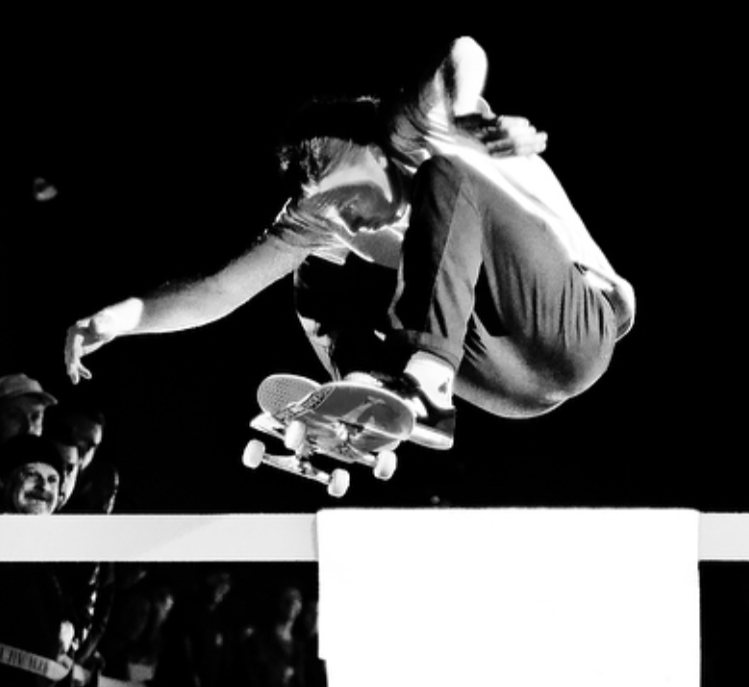
\includegraphics[width=0.2\textwidth]{figure/JakeHayes.png} }}%
    \quad
    \subfloat[\centering Yeadon model in same configuration]{{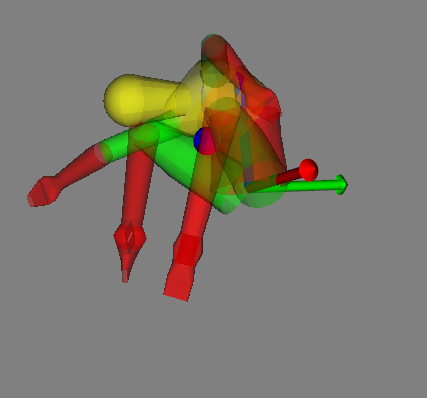
\includegraphics[width=0.2\textwidth]{figure/JakeHayesYeadon.png} }}%
    \caption{Reconstruction of world record ollie} 
    \label{fig:f_record}
    \centering \footnotesize \url{https://theberrics.com/world-record-ollie-footage}$^{1}$%
\end{figure}

We also implement a minimum and maximum foot separation of \SI{0.1}{\meter} and \SI{1.0}{\meter} respectively, along with constraining the skater to always stay on top of the skateboard to eliminate relative errors.
To make sure the feet never leave the skateboard, $s_1$ and $s_2$ are positively bound from the end of the tail and the left pocket of the deck respectively (see fig \ref{fig:FBD}).
The feet can still be in a no contact scenario, as seen in Fig.~\ref{fig:ollie steps}, due to how the friction model is implemented (section~\ref{ss_friction}).

The human kinetics are bounded to the characteristics of a \gls{cmj}.
The \gls{cmj} motion is chosen because it accounts for 76.3\% of the variance in the performance of the ollie~\cite{candotti_lower_2012} and is a reliable assessor of lower-body mechanical power~\cite{barker_relationships_2018}.
During a vertical jump, joint torques, and knee extensor and hip abduction forces all map to one output variable: the \gls{grf}.
As contributions of individual segments cannot be expressed with a point mass model, we bound the \gls{grf} of the \gls{cmj} to capture the realistic kinetics of the human.

We constrain the \gls{rfd} to simulate the leg shortening and lengthening cycle, the maximum force $F_{max}$ keep this within realistic limits, and maximum mechanical power $P = F v_{rel}$ as this also constrains knee extension rate. We obtained numerical values from a study that tested Division-I male soccer players with a mean height of \SI{179.5}{\centi\meter}, weight of \SI{75.5}{\kilo\gram}, and age of 19.65 years~\cite{barker_relationships_2018}. To account for the fact that \citet{barker_relationships_2018} measured two legs simultaneously, we constrain the sum of the forces produced by both legs together. We also constrain the absolute force and power produced by each leg to within realistic physical limits to prevent in and out of phase pushing and pulling of the individual legs.

\subsubsection{Friction Model} \label{ss_friction}
The feet slide along the deck's griptape to drag vertically and level the skateboard. We model both the static and dynamic friction during the foot's sliding on the deck using an approach based on \cite{patel_contact-implicit_2019}.
The relaxed friction formulation in \citet{patel_contact-implicit_2019} is incompatible with the generalized direct collocation formulation in \citet{betts_practical_2010}; it instead uses a special set of complementary constraints formulated using state values at adjacent mesh points to approximate impact as being spread throughout a single mesh section with contact changes only occurring at collocation points.
Application of \cite{patel_contact-implicit_2019} can also result in slow convergence and long compute times, and require a close initial guess~\cite{shield_contact-implicit_2022}.

We modify the method from \cite{patel_contact-implicit_2019} by removing the impact condition between the human and the board, instead assuming that the feet never impact the skateboard and simply exert zero normal force when out of contact.
We start by setting the normal forces of the feet $F_{p1}, F_{p2}$ and the feet accelerations $\ddot{s_1}, \ddot{s_2}$ as control variables.
Foot acceleration is controlled instead of foot location itself to ensure smooth and realistic foot trajectories.
We divide each normal force into a pair of non-negative slack variable representing its positive and negative component, for example $F_{f1} = F_{f1}^+ - F_{f1}^-$.

Friction is then enforced using a set of six path constraints for each foot (shown below for the back foot):
\begin{align} \label{e_frictioncontrol}
    \psi_1 + \dot s_1  &\geq 0 \\
    \psi_1 - \dot s_1  &\geq 0 \\
    \mu F_{p1} - F_{f1}^+ - F_{f1}^- &\geq 0 \\
    (\mu F_{p1} - F_{f1}^+ - F_{f1}^-)\ \psi_1  &= 0 \\
    F_{f1}^+ (\psi_1 + \dot s_1)  &= 0 \\
    F_{f1}^- (\psi_1 - \dot s_1)  &= 0
\end{align}
The first two equations above introduce $\psi_1$, a slack variable representing the magnitude of the relative velocity between the foot and the skateboard $\dot{s}_1$. The third ensures that the positive or negative component of the friction is always smaller than $\mu F_{p1}$, while the fourth ensures that when the foot slides the sum of the positive and negative friction components equal $\mu F_{p1}$. It is important that when sliding in the positive direction, the negative friction component $F_{f1}^- = \mu F_{p1}$ and $F_{f1}^+=0$, and vice versa. This is enforced by the final two path constraints.

\subsubsection{Endpoint constraints} \label{p_endpoints}
Each phase is described with pair of variables describing its initial and final time. Phases are constrained such that phase final times are after phase initial times, phase duration is flexible, and the three phases are sequential.

To ensure the human starts the ollie from a standing position, the vertical forces at the beginning of phase 1 are constrained to equal the body weight.
Switching between the first and second phases occurs when the tail hits the ground.
This is implemented by calculating the impact angle of the skateboard as a function of the parameter values and using this as an endpoint constraint for the first phase.
The other phase transition occurs at the point when the skateboard's vertical velocity is zero.
The ollie landing, and \gls{ocp} final time, is defined by the back wheel touching the ground at a minimum of \SI{0}{\radian} (level) and a maximum of \SI[parse-numbers = false, number-math-rm = \ensuremath]{\frac{\pi}{6}}{\radian} (rotated counterclockwise).

Continuity of all state variables is enforced between phases 1 and 2 and phases 2 and 3. The exceptions are the translational and angular velocity of the skateboard at the boundary between the first two phases. During this collision the ground exerts a normal linear impulse. To calculate speeds after impact, we use a matrix representation method of Newton's impact law~\cite{vallery_heike_advanced_2018} and enforce these as endpoint constraints at the start of phase 2.


\subsection{Solver Configuration}\label{s_settings}
We used an initial transcription mesh involving 30 mesh sections for phases 1 and 2, and 10 mesh sections for phase 3. The optimal trajectory in the first two phases is more nonlinear than the third phase requiring a more dense mesh to be used.
Additionally, settings for the \gls{nlp} and mesh tolerances in Pycollo were set to $1e^{-8}$ and $1e^{-3}$ respectively.

\subsection{Summary}\label{s_summary}
A full mathematical description of the \gls{ocp} definition including all variables, constraints and bounds can be found in \cite{heinen_optimal_2022}, along with the code used to formulate and solve the \gls{ocp}.

%%%%%%%%%%%%%%%%%%%%%%%%%%%%%%%%%%%%%%%%%%%%%%%%%%%%%%%%%%%%%%%%%%%%%%

\section{Results}

We produced our results using Python 3.X.X, Pycollo 0.X.X and Ipopt 3.13.X, on a MacBook Pro with Apple M1 Pro CPU, \SI{16}{\giga\byte} RAM and running macOS Ventura 13.2.1.
All \glspl{ocp} were solved in less than 3 minutes.
We consistently used a null seed initial guess and ensured successful Ipopt and Pycollo exit statuses meeting the desired \gls{nlp} and mesh tolerances specified in section~\ref{s_settings}.

\subsection{Optimal Trajectories and \\Geometries}

\begin{figure*}
    \centering
    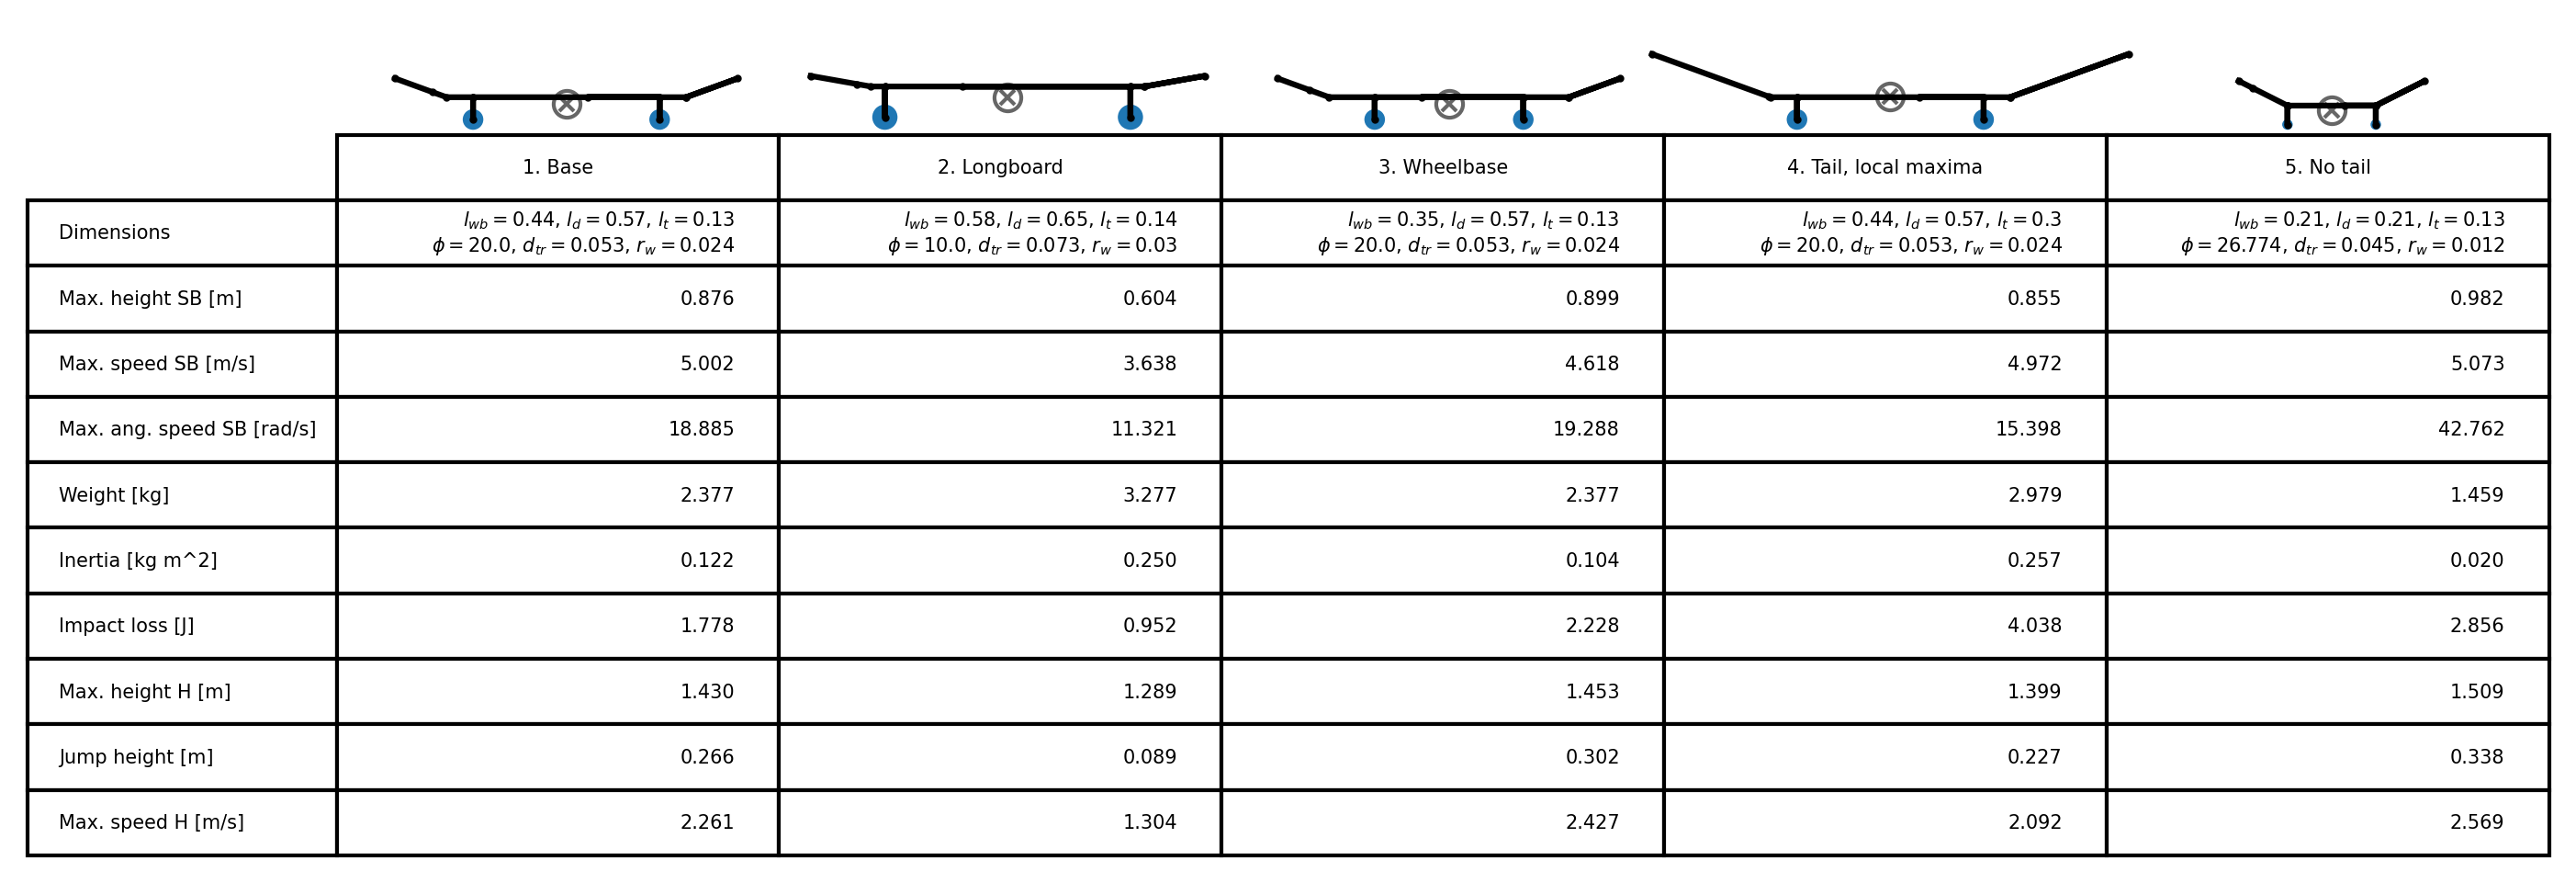
\includegraphics[width=\textwidth]{paper/figure/Results/ResultsTable.png}
    \caption[Results benchmarks]{Key values from the results of five different ollie optimizations: skateboards~1 and 2 are a fixed geometry popsicle skateboard and longboard respectively; skateboard~3 has an optimizable wheelbase; skateboard~4 has an optimizable tail/nose length; and skateboard~5 has an optimizable wheelbase, deck length, tail/nose inclination, truck height, and wheel radius. Mass centers are shown with a cross. Jump height is calculated by subtracting the take-off vertical position of the person from the minimum vertical position. The impact loss is calculated as the difference in skateboard kinetic energy before and after impact}
    \label{fig:resultstable}
\end{figure*}

We present the results of five separate \glspl{ocp}. Schematics of each skateboard and key metrics for each optimized trajectory are shown in figure~\ref{fig:resultstable}. Skateboards~1 and 2 are a popsicle stick (base) skateboard and longboard respectively. The longboards' dimensions are selected to match an arbitrary OEM longboard.\footnote{\url{https://hlcskateboardfactory.com/shape:MB701}} While we performed all possible single parameter optimizations, we only present two here for discussion; skateboards~3 and 4 had their wheelbase and tail length optimized respectively. Finally, skateboard~5 was multi-parameter optimization involving the simultaneous optimization of wheelbase, deck length, tail/nose inclination, truck height, and wheel radius.

You can find animations of the five optimal trajectories in the supplementary material or at \url{youtu.be/jw5DmNnvD7c}.

% All possible single parameter optimizations are performed, the best and worst performing optimizations are presented in Fig.~\ref{fig:resultstable}.4 and \ref{fig:resultstable}.5. are found with a single parameter optimization. Compared to the base skateboard, all single parameter optimization skateboards were able to ollie higher except for the tail length optimization (4). The optimization was able to ollie \SI{0.023}{\meter} higher with a \SI{0.09}{\meter} smaller wheelbase. The tail length optimization did not find a higher maxima which makes it a local maximum per definition, because the base solution is in the solution space of the tail optimization. The cause of hitting a local optimum because of the tail length needs further investigation. We will exclude this optimization for detailed analysis in the next subsection.

% The fifth optimization is found with multiple parameter optimization. The ollie height improved improved by 0.106 [m] compared to the base skateboard. 

%The cause of hitting a local optimum because of the tail length needs further investigation. When the tail length increases the impact loss increases as well. This is logical when thinking of the tail speed $v = \omega \times r$, which means, the larger the distance between the tip of the tail and COM of the skateboard, the larger the local speed at the tail. The larger the speed at the tail, the more momentum is lost during impact, which is the reason for the higher impact losses. The impact loss is dependant on the mass and speed, the higher the mass or the speed, the higher the impact loss will be. For example in the `no $l_t$' (figure \ref{f_multipar}) optimization the angular velocity before impact is more than twice as high compared to the base optimization. But the mass is also 0,878[kg] less. Thus, the large angular velocity causes the impact loss to be higher, but the mass reduction reduces it, only causing a slight gain in impact loss. 

\begin{figure*}
    \centering
    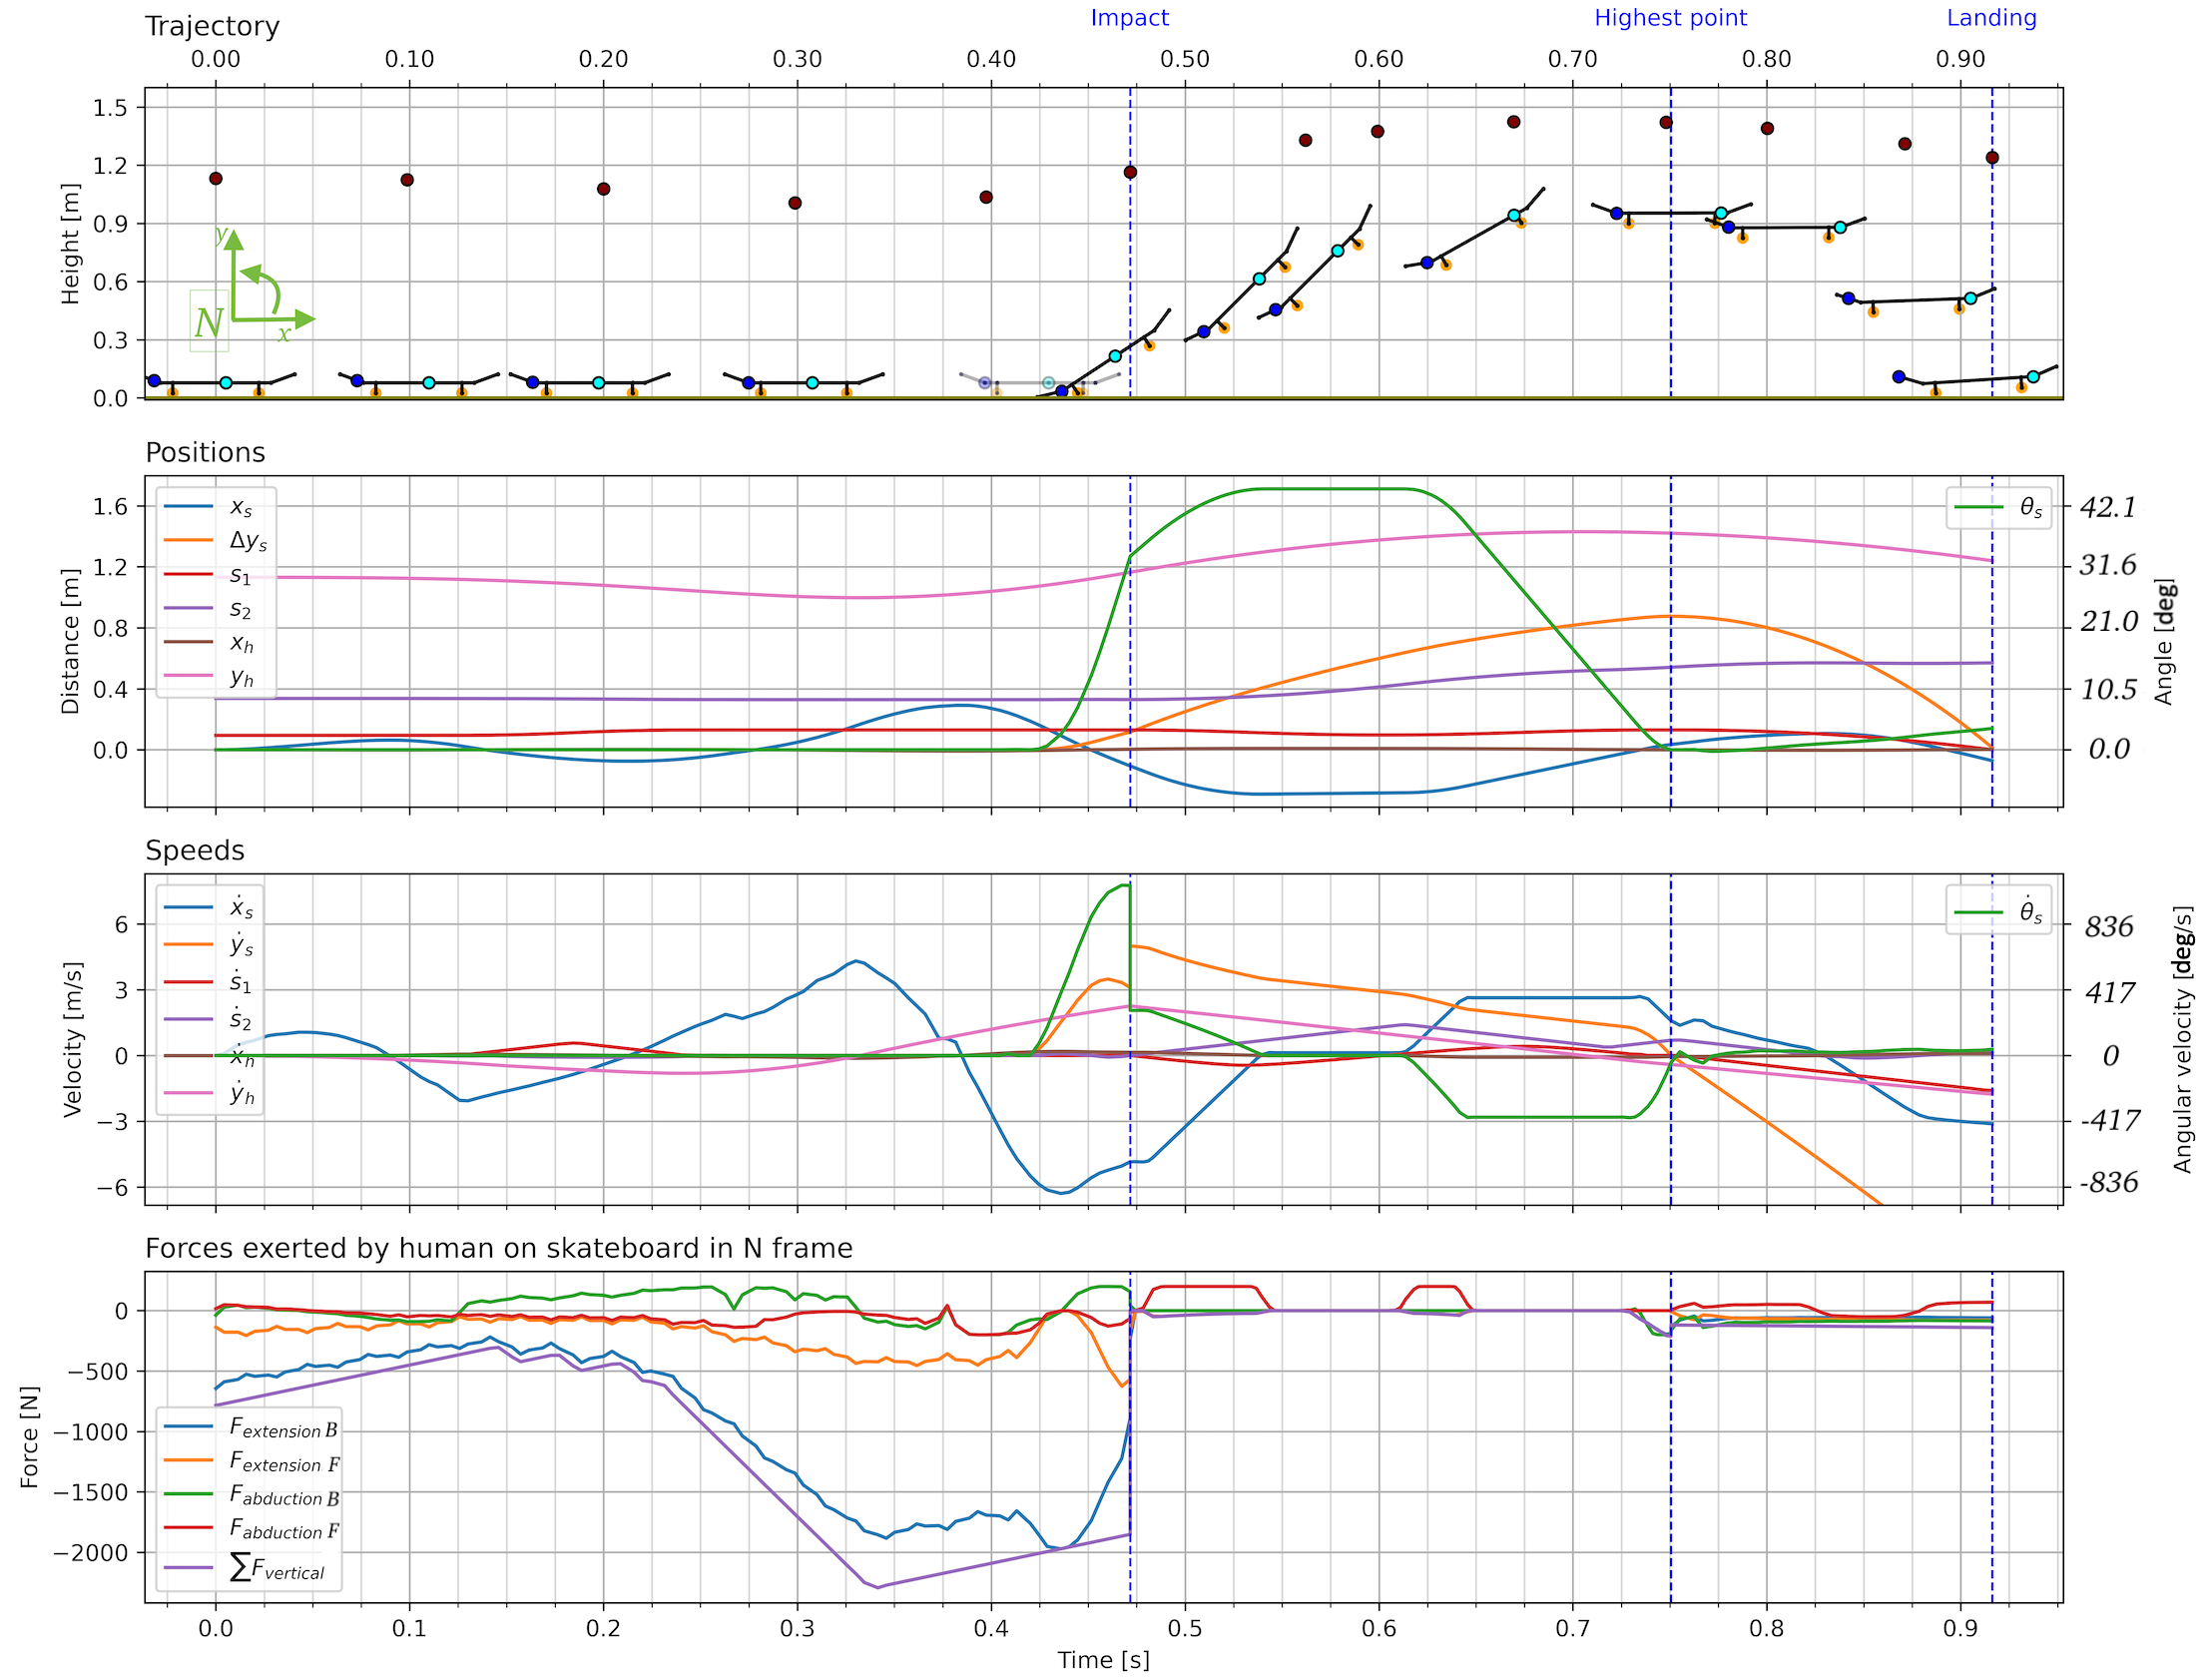
\includegraphics[trim={0cm 0cm 0cm 0cm},clip,width=\textwidth]{paper/figure/Results/data_basedpi600 (1).png}
    \caption[Trajectory, positions, speeds, and forces of base optimization]{\foot
    Detailed trajectory of base skateboard}\label{f_noparameter}
    Graph (1) shows the trajectory of the skateboard, the COM of the human corresponds to the time. (2) are the coordinates of the skateboard and the human over time. (3) are the speeds of skateboard and human over time. (4) are the extension (N-frame y direction - see first plot for frame convention), abduction (N-frame x direction) and sum of extension forces. The blue dotted lines are the phase switches. Time corresponds vertically between graphs. First the human lowers their COM (pink,2) by decreasing vertical force (purple, 4), at minimal human COM height there is maximal force and zero speed (pink,3). Maximal force is almost fully caused by the extension force of the back foot (blue,4). Speed is increased until impact and it reaches maximum speed (pink,3 at impact). Just before impact the skateboard rotates its angle (green,2) from 0 to impact angle. Mid air the speeds are constant except ones effected by gravity (orange,pink,3). The moments forces are exerted the velocities change (t=0.5, t=0.63). The human reaches its highest point before the skateboard. At the highest point force is exerted to `catch' the skateboard. Landing is achieved by stretching and landing on the back wheel
\end{figure*}

\subsubsection{Base skateboard optimization}
We solved the base skateboard \gls{ocp} to demonstrate that the model and optimization methodology produce ollies with realistic kinematics and kinetics.
The optimal trajectory is shown in figure~\ref{f_noparameter} and is very similar to the trajectory shown in figure \ref{fig:ollie steps}.
Initially, the skateboard moves forward relative to the human. Immediately prior to the impact of the tail with the ground, the skateboard rapidly moves backward. 
The back foot is located at the pocket of the skateboard, the point with the lowest velocity of the tail during rotation.
Impact changes the momentum of the skateboard.
In the speeds subplot of figure~\ref{f_noparameter} it is visible that the angular velocity reduces at impact (green line, \SIrange{1082}{286}{\degree\per\second}), while vertical velocity is gained (orange line, \SIrange{3}{5}{\meter\per\second}).

The human controller follows a \gls{cmj} force graph where unloading is from $t=\SIrange{0.0}{0.2}{\second}$, eccentric braking is at $t=\SIrange{0.2}{0.35}{\second}$, and the concentric phase is from $t=\SI{0.35}{\second}$ until impact.
During the concentric phase the vertical velocity (pink line) increases.
The force reduces to comply to the power bound ($P_{leg} = v_{rel} F$) until the human loses contact with the skateboard just before impact.
During upward motion, the vertical velocity of the human gradually decreases due to gravity, reaching it's highest point just before the ollie's peak.
The slopes and maximum of the vertical forces (purple line) are bound by the eccentric (negative) and concentric (positive) \gls{rfd}, and the maximum force permitted.
The optimizer operating at these bounds indicates that maximizing force and power output also maximizes ollie height.

\subsubsection{Longboard optimization}



\subsubsection{Wheelbase optimization}

\begin{figure*}
    \centering
    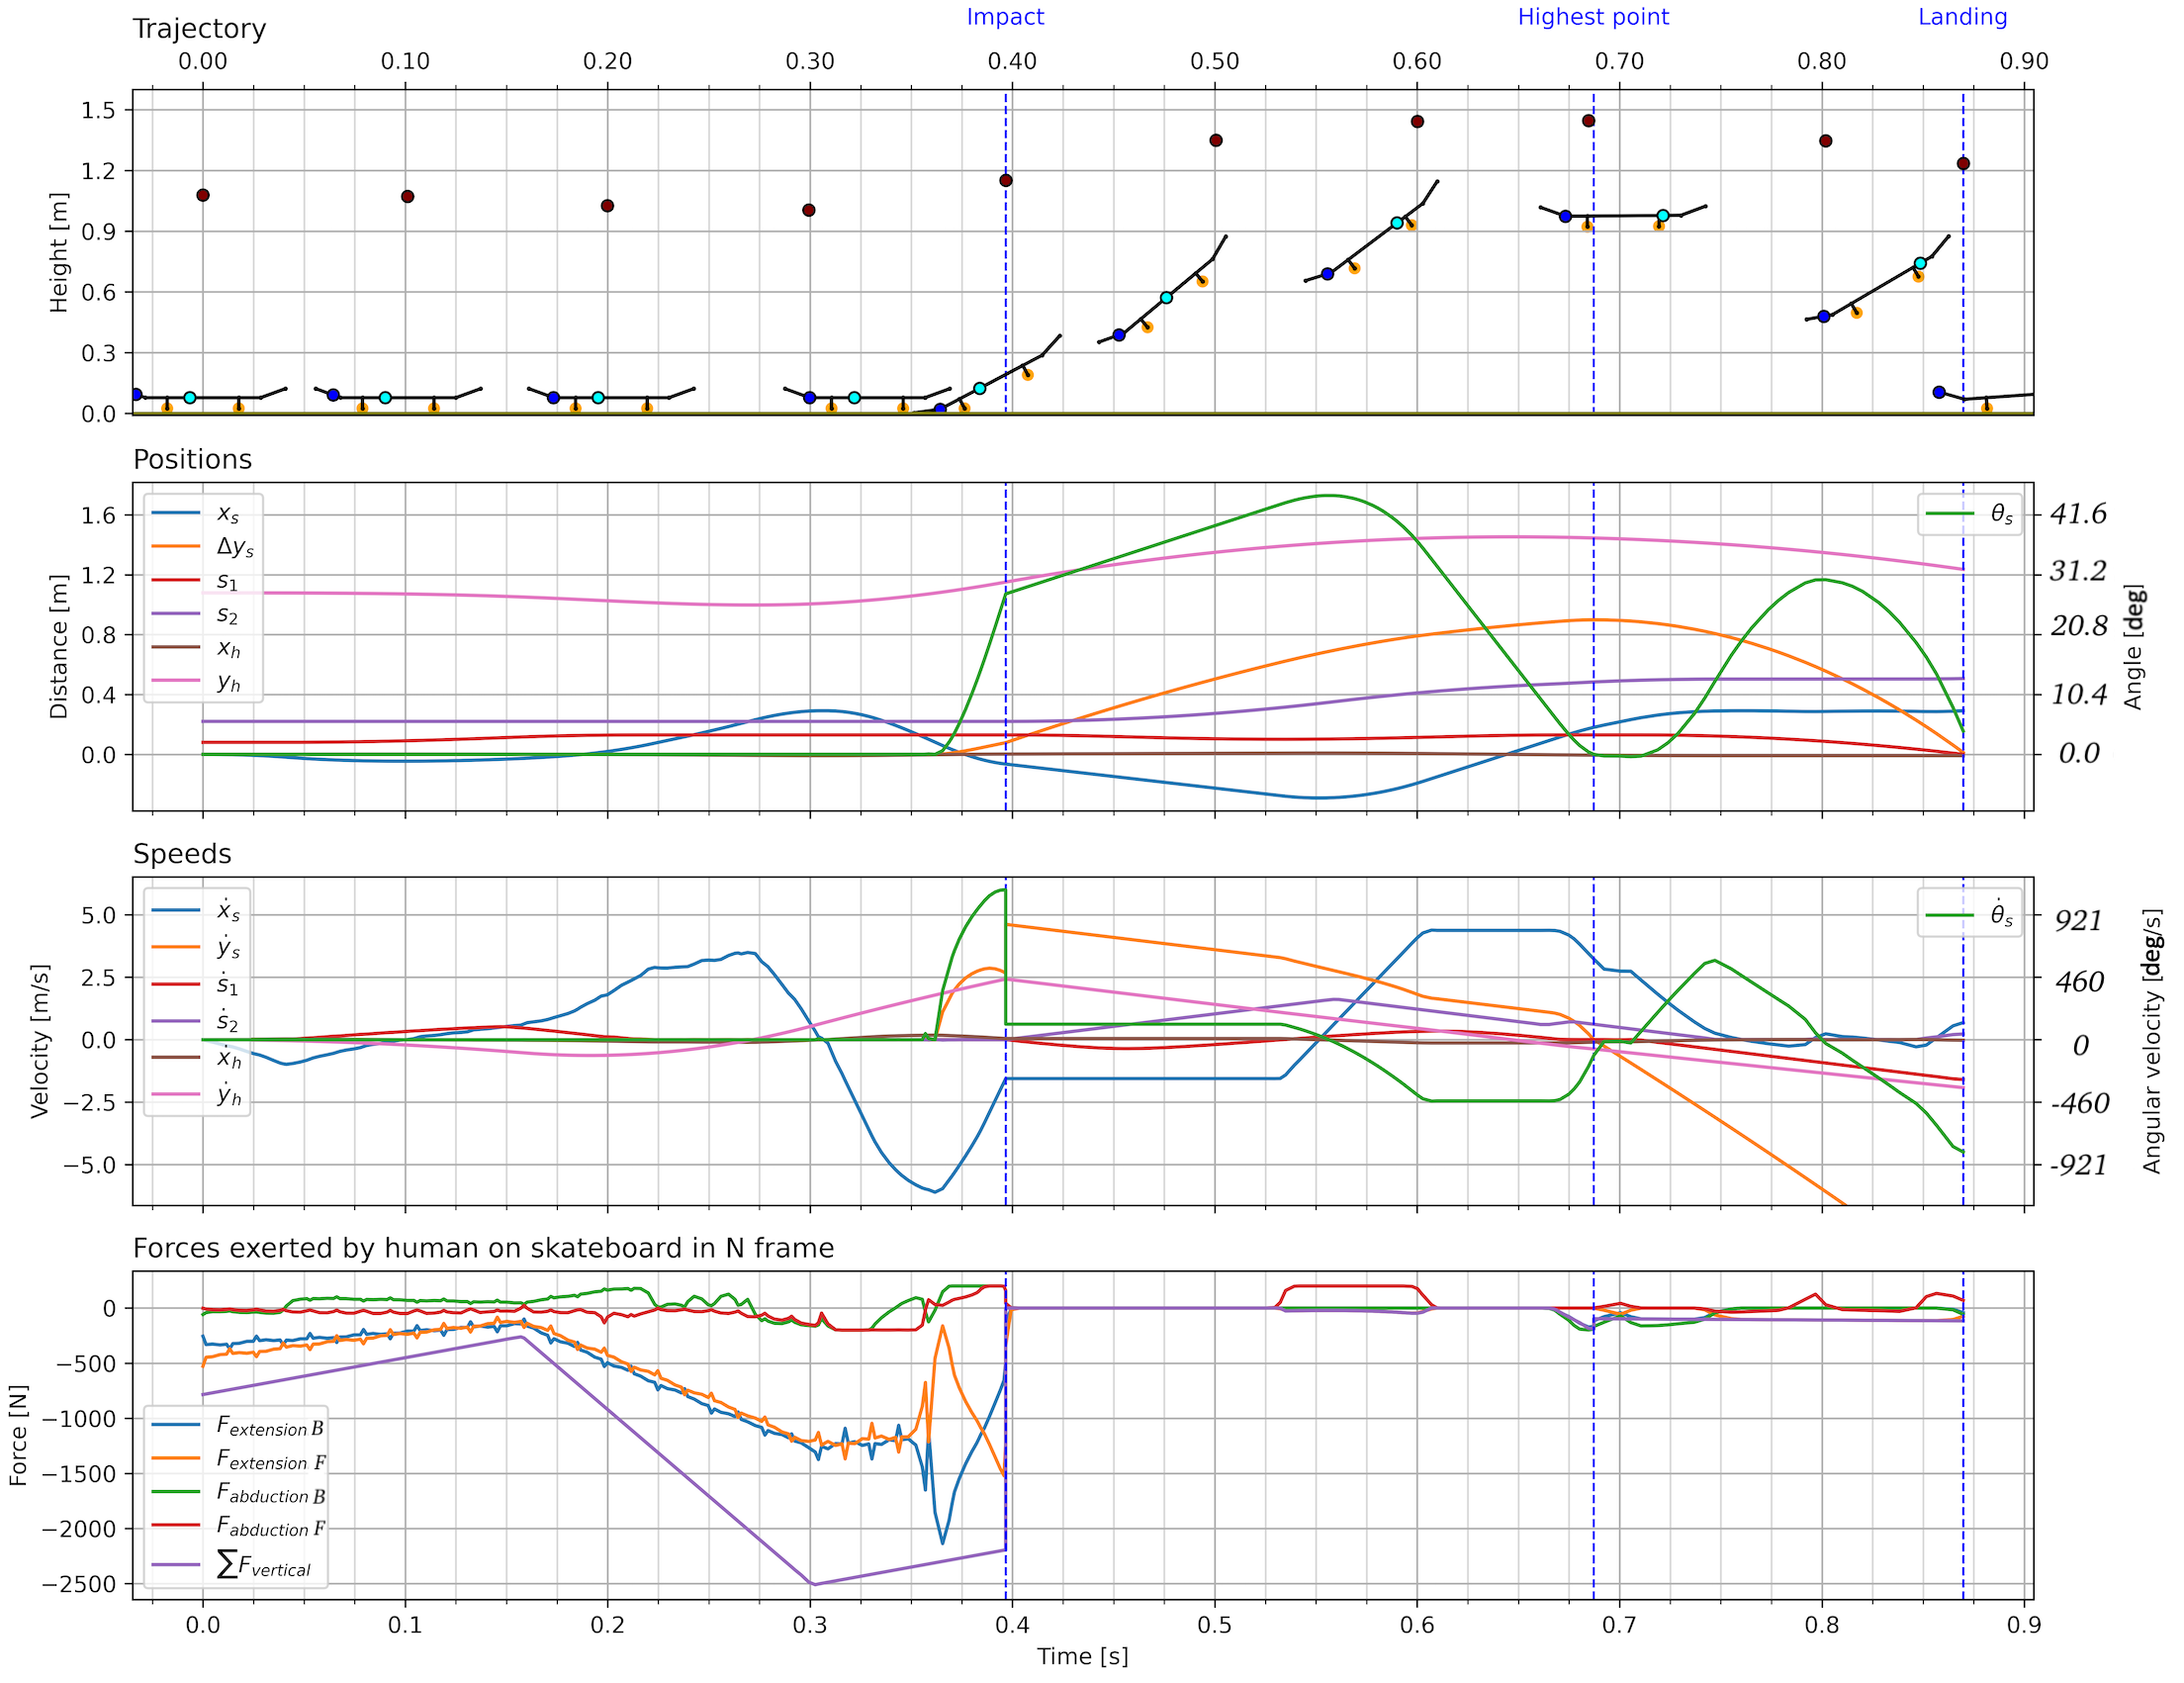
\includegraphics[trim={0cm 0cm 0cm 0cm},clip,width=0.85\textwidth]{paper/figure/Results/data_l_wbdpi600 (1).png}    
    \caption[Trajectory, positions, speeds, and forces for wheelbase optimization]{Detailed trajectory of optimized wheelbase}\label{f_wheelbase}
    Corresponds to result 3. Wheelbase in Fig.~\ref{fig:resultstable}. 0.09[m] smaller wheelbase compared to base, 0.023[m] higher ollie. Three striking differences, the first is that the jumping force is now equally dependant on the back and front extension force (blue,orange,4), the second is that there is only one force peak between impact and highest point. The third striking part is that the skateboard rotates before landing (t=0.8)

    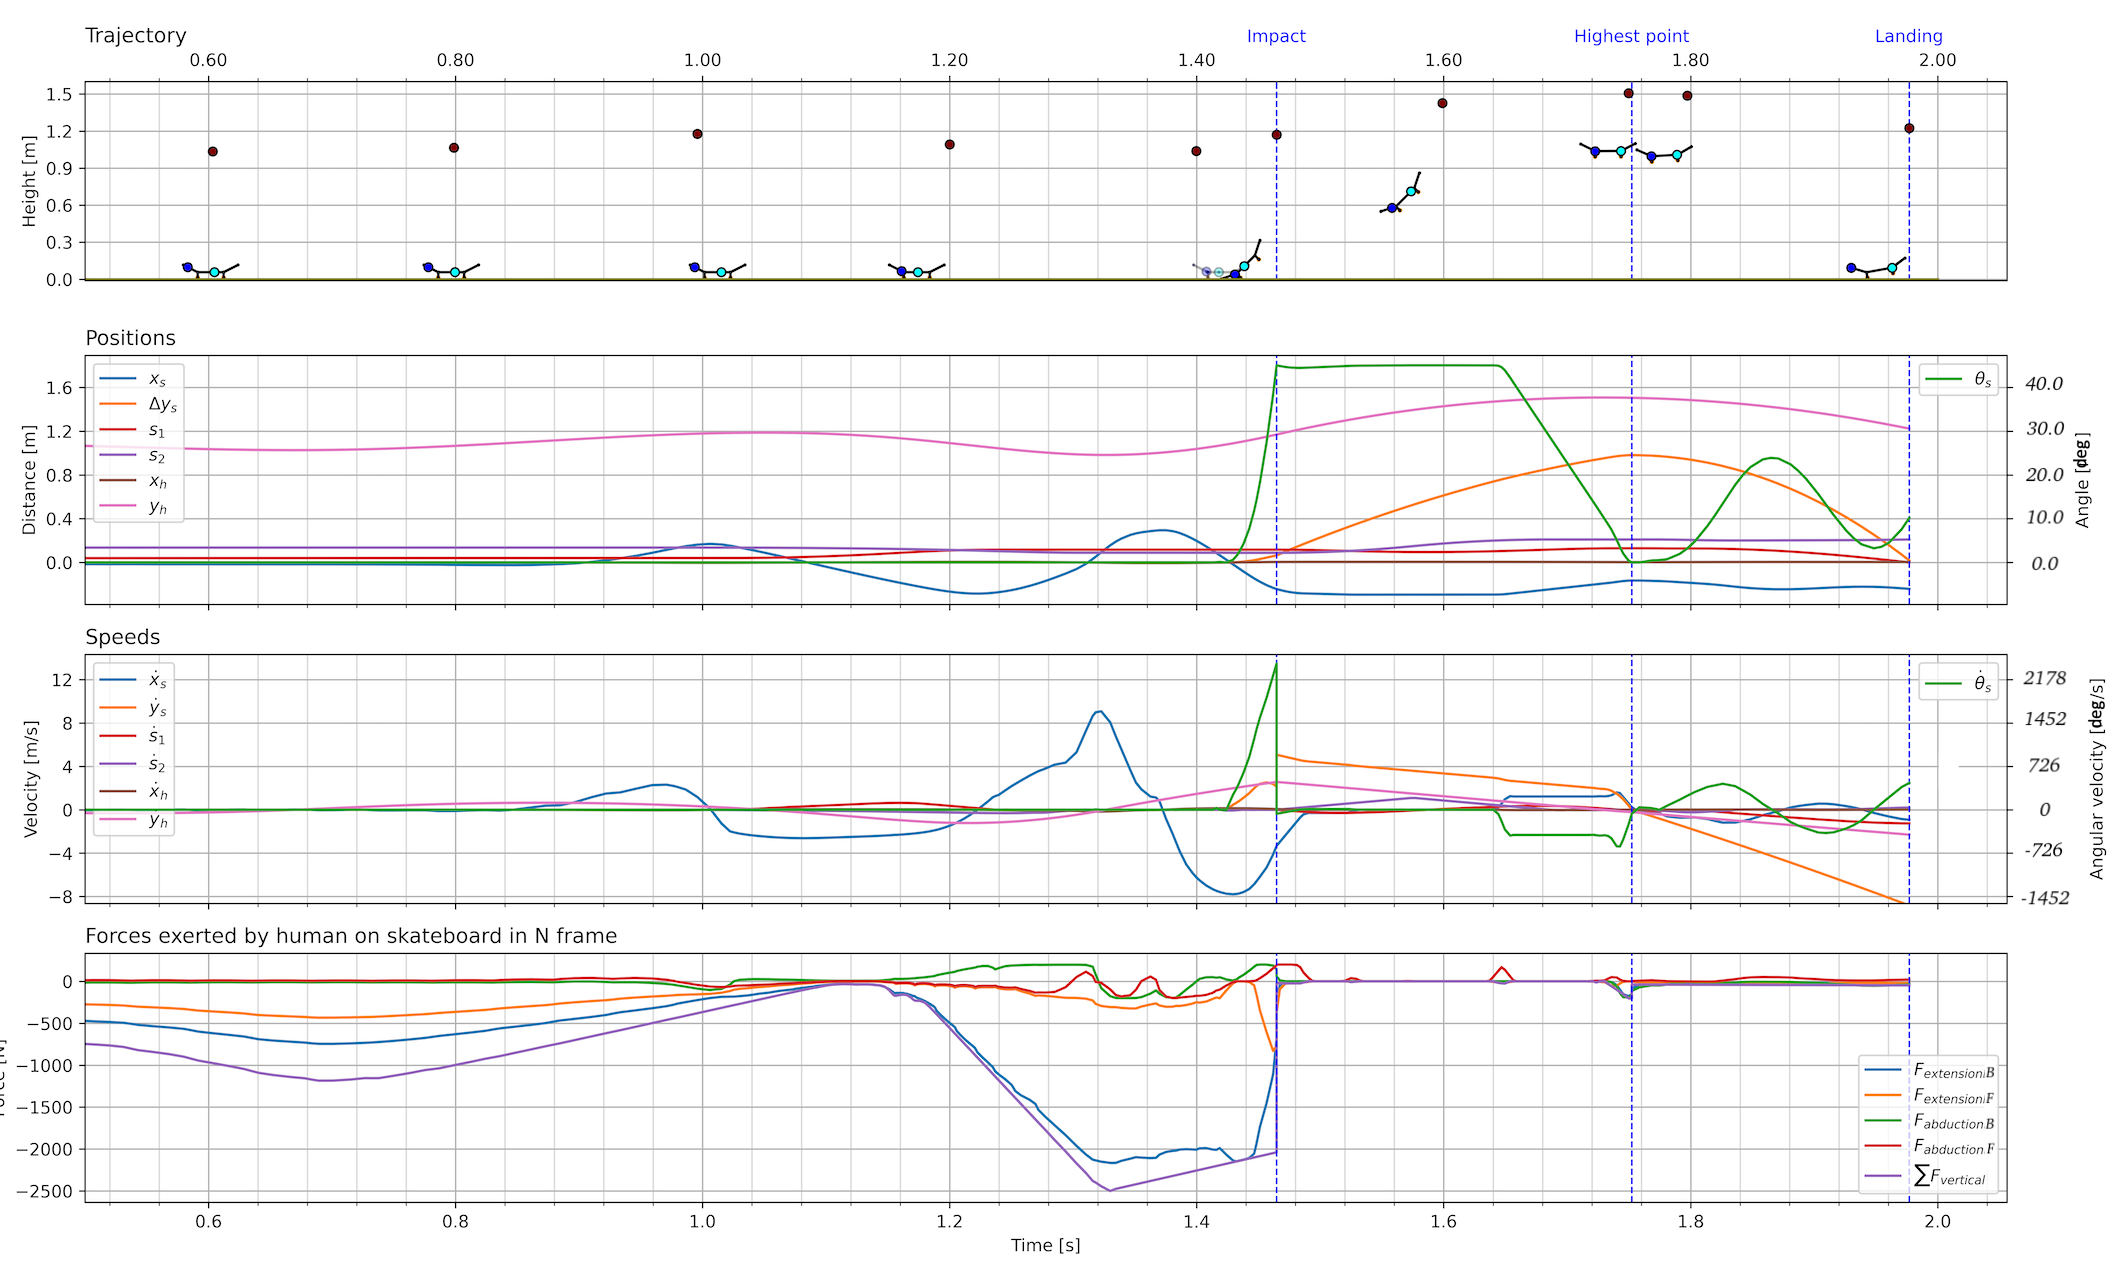
\includegraphics[trim={0cm 0cm 0cm 0cm},clip,width=0.85\textwidth]{paper/figure/Results/data_no_taildpi600 (1).png}
    \caption[Trajectory, positions, speeds, and forces for `all except tail length' optimization]{Detailed trajectory of optimization of all parameters except the tail}\label{f_notail}
    Optimization `no $l_t$'. Corresponds to result 5. No tail in Fig.~\ref{fig:resultstable}
\end{figure*}

Most of the phenomena seen in the base optimization are also visible for this optimization. The first difference is visible in the force plot in Fig~\ref{f_wheelbase}. The sum of the vertical forces (purple line) does not stagger when unloading. Secondly, a higher angular velocity is achieved. The front foot is at equal distance from the wheel having perfect balance. At this position both legs can exert equal force without rotating the board during eccentric braking ($t=0.15 - 0.3$). Shortly before the impact, the front foot (orange line forces) releases pressure and the back foot pushes down to create a maximal momentum about the back axis creating a steep increase in angular velocity. The decreased wheelbase causes the impact angle to be lower and the angular velocity near zero just after impact (green lines positions and speeds). No control is needed while gaining height. While the front foot is in a sliding motion, the foot pushes down on the board at $t=0.53$. This is almost enough to level the board out at the highest point. But the negative angular rotation caused by this push is caught with the back foot making sure the board is leveled at the highest point.



\subsection{No tail}
This skateboard is significantly easier to rotate due to the lower inertia and mass ($I_s = 0.02 [kg m^2]$ compared to $0.122 [kg m^2]$ and $m_s = 1.459 [kg]$ compared to $2.377 [kg]$, seen in Fig.~\ref{fig:resultstable}). With the same amount of force over time the angular velocity is twice as high (green line speeds). The human jumps highest with this skateboard setup. With this setup the skateboarder is able to jump almost solely from its back foot (blue line forces) due to the fact that the foot is located almost exactly above the back wheel such that there is no or little momentum created about the back axis. 

\section{Discussion}
The simulated ollie resembles reality. Longboard complies with the real life scenario and the optimization shows a 31\% decrease in ollie height compared to the base. Without any motion cues, the optimizer is able to replicate the ollie motion, with almost all phenomena seen in figure~\ref{fig:ollie steps}. The optimizer shows that the human first jumps, then slams the skateboard to the ground, slides the front foot over the deck to drag it up and level it out and catches the skateboard with the back foot at the highest point. This is very close to reality. All results show high similarities to a \gls{cmj} \gls{grf}. The sum of the human kinetics are well bound and show constant results. The point mass model is able to show valid results and is insightful for the dynamics, kinetic output and human movement. In an ollie \gls{grf}, the impulse from the skateboard hitting the ground is roughly \SI{5}{\joule}~\cite{determan_kinetics_2006}, which is of the same order of magnitude as the found impact losses in figure~\ref{fig:resultstable}.

Lower inertia and skateboard mass is beneficial for ollie height. In all parameter optimizations that improved ollie height compared to the base, a reduction in mass and inertia is found. The main differences are found in the weight and inertia reduction which could be the main `drive' of the single parameter optimization. Which indicates that inertia and weight reduction is a positive influence for ollie height. Dynamically this makes sense because with lower mass and inertia values it easier to lift and rotate the skateboard.

Popsicle stick skateboard is close to optimum and slight changes due to preference will not influence the ollie height significantly. The best performing single parameter optimization was able to ollie only 0.023[m] higher. When multiple parameters are changed the ollie height increased significantly (0.106 [m]), but the shapes are completely different from a popsicle stick skateboard. If skateboarding will keep the popsicle stick skateboard as standard due to the fact that other tricks need to be performed other than the ollie, not much can be changed to the skateboard to optimize it. If the skateboard will change completely, the ollie height could be improved. The wheelbase effects the ollie height the most of all single parameter optimizations, which could be a promising outcome since it does not influence the board shape which is crucial for other tricks.

A fundamentally different simplified contact implicit optimization is made. The relaxed formulation by Patel et al.~\cite{patel_contact-implicit_2019} has been simplified by restating the contact definition. Static and dynamic friction is achieved with the ability to have contact implicit events. The simplification leads to quicker convergence and works with a null seed initial guess. The ollie optimization by Shield et al.~\cite{shield_contact-implicit_2022} was without a parameter optimization of the skateboard. This optimization took 43 minutes to solve, and accurate initial guesses were needed for feasible results. Our code solved under 3 minutes including derivation of the Equations of Motion and all constraints, the time to transcribe the problem and to solve in IPOPT. This was all done without initial guesses and solved optimally.



Tail length optimization leads to local maxima. The optimization wants to maximize tail length dispite the lower ollie height. In real life a longer tail length would cause a higher energy dissipation due to more bending during impact. A plausible cause for these local maxima is that impact loss is of too little effect. When a human jumps, the order of magnitude of the amount of energy necessary to go up is in the order of $10^3$. The dissipation of energy during impact is in the order of $10^-1$. This means that the impact loss could be of so little effect to increasing ollie height that the solution space has become very flat. The model does capture the increase impact loss in figure \ref{fig:resultstable}, but it is not sufficient to influence the solution. All other solutions are not granted to be global optima either. Direct collocation does not guarantee global optima. Though, finding higher outcomes than the base optimization is still valuable for interpreting performance through geometrical dimensions.

In future research it is advised to implement a normal force acting on the front wheel during the preparation phase. The front foot had to counteract the rotation created by the back foot. In real life the front foot could have been on any location without causing a counter clockwise rotation due to the compensation of the normal force. This could be a reason why the force graphs are spikey, since the optimization wit holds another difficulty; balancing the board while ollieing.
 
% Nine out of eleven optimal skateboard geometries found higher ollies compared to the popsicle stick skateboard. None of these solutions is proven a global optimum, but the improvement to the base skateboard is something that performs better. Skateboard builders should try to implement found geometries and test empirically if they will improve ollie height. These geometries could be a tool to alter existing skateboards and let athletes jump higher. The kinetic and kinematic constraints are of a specific person. The geometries might be dependent on the human capabilities. Empirical testing is necessary to prove that this finding is true in a real life ollie. I successfully solved the ollie optimization problem with a geometry optimization. Compared to others Shield et al. \cite{shield_contact-implicit_2022} who solved an optimization problem for the ollie, my optimization was faster (3 min vs. 43 min), included an geometry optimization, and had a more difficult objective function. The Shield optimization was was set at a fixed ollie height and needed motion tracking to solve optimally. My optimization had a null seed initial guess, with an objective function that maximized ollie height. Such objective functions are generally hard to solve, for example in \cite{nitschke_efficient_2020} first tracking data needs to be implemented to solve a more difficult objective. Step by step less data can be used to solve for an more difficult objective. In the case of this paper, the solution is found without any tracking data and a difficult objective function. 

\section{Conclusions}

\section{Acknowledgements}

\section{Statements and Declarations}
\small
\noindent\textbf{Conflicts of interest} There has been no conflict of interest with the
authors involved in this work. \\

\noindent\textbf{Open Access} This article is licensed under a Creative Commons Attribution 4.0 International License, which permits use, sharing, adaptation, distribution and reproduction in any medium or format, as long
as you give appropriate credit to the original author(s) and the source,
provide a link to the Creative Commons licence, and indicate if changes
were made. The images or other third party material in this article are
included in the article's Creative Commons licence, unless indicated
otherwise in a credit line to the material. If material is not included in
the article's Creative Commons licence and your intended use is not
permitted by statutory regulation or exceeds the permitted use, you will
need to obtain permission directly from the copyright holder. To view a
copy of this licence, visit http://creativecommons.org/licenses/by/4.0/.

\bibliographystyle{sn-basic}
\bibliography{references}

\end{document}
